\documentclass[DM,toc,lsstdraft]{lsstdoc}
% lsstdoc documentation: https://lsst-texmf.lsst.io/lsstdoc.html
\usepackage{geometry}
\usepackage{longtable,booktabs,graphicx}
\usepackage{enumitem}
\usepackage{arydshln}

% Generated by Makefile
\input{meta}

% Package imports go here.

% Local commands go here.

% If you want glossaries, uncomment:
% \input{aglossary.tex}
% \makeglossaries

\title{Characterization Metric Report: Science Pipelines Version 27.0.0}
% \setDocSubtitle{Optional subtitle}

\author{%
Jeff Carlin
}

\setDocRef{DMTR-431}
\setDocUpstreamLocation{\url{https://github.com/lsst-dm/DMTR-431}}
\date{\vcsDate}
% \setDocCurator{The Curator of this Document}

\setDocAbstract{%
This brief report describes measurements of data quality metrics that were carried out for release v27.0.0 of the LSST Science Pipelines. The report for the previous version can be found in \citedsp{DMTR-421}.
}

% Revision history.
% Order: oldest first.
% Fields: VERSION, DATE, DESCRIPTION, OWNER NAME.
% See LPM-51 for version number policy.
\setDocChangeRecord{%
  \addtohist{}{2024-06-05}{Unreleased.}{Jeff Carlin}
  \addtohist{1.0}{2024-08-06}{Document issued; DM-44586.}{Jeff Carlin}
}

\begin{document}

\maketitle

In this report, we characterize the performance of the Rubin Observatory Science Pipelines Version 27.0.0. We illustrate the performance via metrics that are measured on the HSC-RC2 dataset. RC2 consists of 3 tracts of data taken from the HSC-SSP survey, and selected to provide a means of testing various ``pathological'' cases (e.g., difficult astrometric solutions, extremely good seeing that does not provide a well-sampled PSF, difficult fields for deblending, and large galaxies, among others). These three tracts each contain between 112--149 visits split between the HSC-G, HSC-R, HSC-I, HSC-Z, and HSC-Y (\emph{grizy}) filters.

Between w\_2023\_32 (the source for pipelines version 26) and w\_2024\_16 (v27 source), most major changes in the science pipelines have been in supporting packages and not to algorithms that dramatically affected the Data Release processing metrics. For example, a new \href{https://pipelines.lsst.io/modules/lsst.source.injection/index.html}{source\_injection} package is now provided to enable injection of synthetic sources into images produced by the pipelines. As of v27, the streak-detection algorithm introduced in v21 is applied during single-frame measurement. In the next release, it will be moved to operate on image differences instead of direct images. This algorithm masks pixels affected by streaks (e.g., satellites or other trailed sources of non-astrophysical origin). Previously, streaks were only removed during coaddition. Another recent change is the adoption of a moments-based star/galaxy classifier rather than the previous binary (i.e., "yes/no") classifier that depended on comparing galaxy model fluxes with PSF fluxes. The moments-based classifier is applied during the characterization and calibration steps of single-frame processing. While the new classifier slightly changes which stars get selected as potential calibrators, its effects on data quality metrics are extremely minor (see \href{https://rubinobs.atlassian.net/browse/DM-39203}{Jira ticket DM-39203} and \href{https://rubinobs.atlassian.net/browse/DM-42663}{DM-42663}). It does, however, slightly affect the selection of candidate stars for PSF fitting and thus has a minor effect on the resulting PSFs -- the effects of this are still under investigation.

Additional new features in this release include:
\begin{itemize}
    \item To limit runtime, the number of stars passed to the PSF determiner and to the PSF matcher within image subtraction is capped.

    \item The implementation of the Pan-STARRS ``pattern continuity'' algorithm, previously specific to the HSC camera geometry, has been generalized to handle all CCD geometries. This algorithm forces the background at the boundaries between amps to be continuous. Now that it runs on LSSTCam geometry, it can improve background models and validate LSSTCam gain stability and instrument signature removal.

    \item The default DRP pipeline switched to using the \href{https://github.com/lsst/scarlet_lite}{scarlet\_lite} standalone package. This package implements the fast and robust single-pixel-scale version of Scarlet.

    \item The astrometric fitting task may now be run in ``global mode,'' which uses all available visits across the survey to produce one global solution in addition to the prior method of independent solutions per tract. It now accepts the outputs from the FitAffineWcsTask fitter as initial estimates, returns uncertainty estimates on the final astrometric model, and is more robust.

    \item The Alert Production pipeline switched to the new CalibrateImageTask instead of the former CharacterizeImageTask and CalibrateTask.

    \item The synthetic source injection package is now included in lsst\_distrib. This update is accompanied by documentation that provides detailed instructions on how to use it and an FAQ.
\end{itemize}

Photometry and astrometry metrics reported here were calculated using the \href{https://github.com/lsst/analysis_tools}{analysis\_tools} package, which is part of the standard pipeline distribution. The \texttt{analysis\_tools} package builds on and supersedes \href{https://github.com/lsst/faro}{faro} (\citeds{DMTN-211}), which has been used for the past few years. The calculation of most metrics reported in this Report is unchanged between the two packages, though minor differences are to be expected because of fundamental differences in the underlying data-handling frameworks. As discussed in the next section, the photometric outlier fraction PF1 has been updated relative to previous pipeline release versions in order to fix a mistake in how the calculation was implemented. We are actively working on a revised definition of the residual ellipticity correlation metrics TE1 and TE2, to be implemented in \texttt{analysis\_tools}. Because this work is still in progress, the ellipticity metrics reported here are calculated by \texttt{faro} in the same manner as previous versions of the Characterization Metric Report.

The metric calculation pipelines from \texttt{analysis\_tools} were run on the three RC2 tracts to derive the photometry and astrometry metrics, and \texttt{faro} to calculate the shape metrics that are reported here. We exclude the two astrometry metrics (AM3 and AF3) that concern residuals on 200-arcminute scales, since the individual tracts of RC2 do not span large enough spatial scales to enable these measurements.

For comparison, we provide the \SRD required ``design'' value of each Key Performance Metric (KPM) as defined in the Science Requirements Document \citedsp{LPM-17}. For the ellipticity correlation metrics, there are specifications only for \emph{r} and \emph{i} bands. The \emph{ugzy}-band measurements are of interest primarily for historical tracking.

Some KPMs (e.g., PF1, AF1, AF2) involve thresholds that are different for ``design'', ``minimum'', and ``stretch'' specifications. Metrics in this report are all compared to the ``design'' thresholds. The assessment of these KPMs would be different if evaluated against different thresholds.

\begin{figure}[!t]
  \centering
  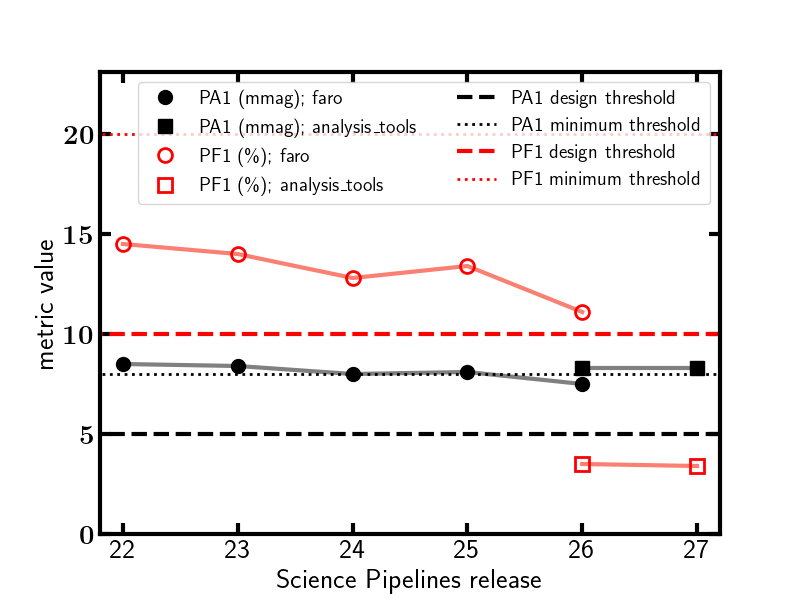
\includegraphics[width=0.6\textwidth, trim=0.0in 0.0in 0.0in 0.0in, clip]{figures/photom_metrics_v27_with_thresholds.png}
  \caption{Photometry metrics PA1 (photometric repeatability) and PF1 (percentage of measurements exceeding the outlier threshold) measured in the $r$-band. The figure shows the values of these metrics as measured with \texttt{faro} in versions 22-26 of the LSST Science Pipelines as circles, compared against the SRD requirements (for both the ``design'' and ``minimum'' thresholds). The measurements from \texttt{analysis\_tools} in versions 26-27 of the Science Pipelines are shown as squares. The measured values of both metrics are unchanged between the two most recent releases (v26 and v27). The algorithm to calculate PA1 is unchanged between \texttt{faro} and \texttt{analysis\_tools} (though because of differences in software architecture, it is expected that we would see minor differences in their outputs), and the metric differs by only a small offset between the two versions calculated in v26. However, while porting the PF1 metric to \texttt{analysis\_tools}, we discovered an error in the method of calculation (see the text for details). Fixing this error reduced the value of PF1 significantly.}
  \label{fig:phot_metrics}
\end{figure}

\section{Summary of performance metrics}

As noted previously, we now report metrics calculated by the \texttt{analysis\_tools} package, which improves upon the \texttt{faro} tools we had been previously using for calculation of data quality metrics. The plots in this Report include metrics from both \texttt{analysis\_tools} and \texttt{faro} for historical continuity, but future data processing campaigns will not run the \texttt{faro} tasks. One significant change is evident when comparing the outputs of the two frameworks on the v26 dataset: in Figure~\ref{fig:phot_metrics}, PF1 is much smaller as measured by \texttt{analysis\_tools} than from \texttt{faro}. This is expected, as we discovered an error in the calculation that was fixed when porting the PF1 metric from \texttt{faro} to \texttt{analysis\_tools} (see \href{https://rubinobs.atlassian.net/browse/DM-39332}{Jira ticket DM-39332} for details). The previous version had been calculating the outlier fraction relative to a fixed value of 15 mmag, while the metric is intended to be the fraction of outliers \textit{more than 15 mmag from the median} photometric repeatability. The changes on DM-39332 have brought the PF1 metric's calculation in line with the description in the DMSR, resulting in a value that is well beneath the design threshold for PF1.

As noted in the previous section, most of the major changes between versions 26 and 27 of the pipelines are related to improvements in supporting packages (e.g., the \texttt{source\_injection} tools) and instrument-specific modifications. Most of the data processing algorithms in the Science Pipelines are virtually unchanged between versions 26 and 27, so the data quality metrics should also be similar. Indeed, the photometry metrics (Section~\ref{photometric-performance}) are unchanged, and the astrometry metrics (Section~\ref{astrometric-performance}) show only minor changes (particularly, slight improvements in the outlier fractions AF1 and AF2). These minor changes in the astrometric outlier fractions were expected following the implementation of \href{https://rubinobs.atlassian.net/browse/DM-43238}{Jira ticket DM-43238}, which provided some speed-ups to execution by down-sampling the pairs of stars used for metric calculations to 100,000 pairs (down from many millions in some cases). Vectorization of the calculations necessitated comparing to the mean rather than the median repeatability for AF1 and AF2, which is the reason for the slight change in their values. Because these outlier fractions were already well below their required thresholds, the change was deemed acceptable given the massive speed-up in calculation that it achieved.
The ellipticity correlation metrics (Section~\ref{ellipticity-correlations}) show only a small difference between Release 26 and 27 for TE1 (median ellipticity residual correlations at 1 arcminute scales), but the TE2 (5-arcminute scales) value has nearly doubled.


\section{Photometric Performance}\label{photometric-performance}
% NOTE: In v28, add the calib flux repeatability!

These photometric performance metrics are defined in LSS-REQ-0093 (\citeds{LSE-29}) and Table 14 of \citeds{LPM-17}. Values in this table represent the mean of the results reported by \texttt{analysis\_tools} for the three tracts in RC2.

Any entries left blank are those for which we do not have data in the given filter for that dataset.

\begin{longtable}[]{@{}llllll@{}}
\toprule
\begin{minipage}[b]{0.12\columnwidth}\raggedright\strut
Metric\strut
\end{minipage} & \begin{minipage}[b]{0.06\columnwidth}\raggedright\strut
Unit\strut
\end{minipage} & \begin{minipage}[b]{0.14\columnwidth}\raggedright\strut
SRD Requirement -- Design\strut
\end{minipage} & \begin{minipage}[b]{0.12\columnwidth}\raggedright\strut
Release 26 Value (RC2) \strut
\end{minipage} & \begin{minipage}[b]{0.12\columnwidth}\raggedright\strut
Release 27 Value (RC2) \strut
\end{minipage} & \begin{minipage}[b]{0.17\columnwidth}\raggedright\strut
Comments\strut
\end{minipage}\tabularnewline
\midrule
\endhead
\begin{minipage}[t]{0.12\columnwidth}\raggedright\strut
PA1: \emph{u}\strut
\end{minipage} & \begin{minipage}[t]{0.06\columnwidth}\raggedright\strut
mmag\strut
\end{minipage} & \begin{minipage}[t]{0.14\columnwidth}\raggedright\strut
\(\leq 7.5\)\strut
\end{minipage} & \begin{minipage}[t]{0.12\columnwidth}\raggedright\strut
--- \strut
\end{minipage} & \begin{minipage}[t]{0.12\columnwidth}\raggedright\strut
--- \strut
\end{minipage} & \begin{minipage}[t]{0.17\columnwidth}\raggedright\strut
No data\strut
\end{minipage}\tabularnewline
\begin{minipage}[t]{0.12\columnwidth}\raggedright\strut
PA1: \emph{g}\strut
\end{minipage} & \begin{minipage}[t]{0.06\columnwidth}\raggedright\strut
mmag\strut
\end{minipage} & \begin{minipage}[t]{0.14\columnwidth}\raggedright\strut
\(\leq 5.0\)\strut
\end{minipage} & \begin{minipage}[t]{0.12\columnwidth}\raggedright\strut
7.2 \strut
\end{minipage} & \begin{minipage}[t]{0.12\columnwidth}\raggedright\strut
7.9 \strut
\end{minipage} & \begin{minipage}[t]{0.17\columnwidth}\raggedright\strut
\strut
\end{minipage}\tabularnewline
\begin{minipage}[t]{0.12\columnwidth}\raggedright\strut
PA1: \emph{r}\strut
\end{minipage} & \begin{minipage}[t]{0.06\columnwidth}\raggedright\strut
mmag\strut
\end{minipage} & \begin{minipage}[t]{0.14\columnwidth}\raggedright\strut
\(\leq 5.0\)\strut
\end{minipage} & \begin{minipage}[t]{0.12\columnwidth}\raggedright\strut
8.3\strut
\end{minipage} & \begin{minipage}[t]{0.12\columnwidth}\raggedright\strut
8.3\strut
\end{minipage} & \begin{minipage}[t]{0.17\columnwidth}\raggedright\strut
\strut
\end{minipage}\tabularnewline
\begin{minipage}[t]{0.12\columnwidth}\raggedright\strut
PA1: \emph{i}\strut
\end{minipage} & \begin{minipage}[t]{0.06\columnwidth}\raggedright\strut
mmag\strut
\end{minipage} & \begin{minipage}[t]{0.14\columnwidth}\raggedright\strut
\(\leq 5.0\)\strut
\end{minipage} & \begin{minipage}[t]{0.12\columnwidth}\raggedright\strut
8.6\strut
\end{minipage} & \begin{minipage}[t]{0.12\columnwidth}\raggedright\strut
8.7\strut
\end{minipage} & \begin{minipage}[t]{0.17\columnwidth}\raggedright\strut
\strut
\end{minipage}\tabularnewline
\begin{minipage}[t]{0.12\columnwidth}\raggedright\strut
PA1: \emph{z}\strut
\end{minipage} & \begin{minipage}[t]{0.06\columnwidth}\raggedright\strut
mmag\strut
\end{minipage} & \begin{minipage}[t]{0.14\columnwidth}\raggedright\strut
\(\leq 7.5\)\strut
\end{minipage} & \begin{minipage}[t]{0.12\columnwidth}\raggedright\strut
6.7\strut
\end{minipage} & \begin{minipage}[t]{0.12\columnwidth}\raggedright\strut
6.7\strut
\end{minipage} & \begin{minipage}[t]{0.17\columnwidth}\raggedright\strut
\strut
\end{minipage}\tabularnewline
\begin{minipage}[t]{0.12\columnwidth}\raggedright\strut
PA1: \emph{y}\strut
\end{minipage} & \begin{minipage}[t]{0.06\columnwidth}\raggedright\strut
mmag\strut
\end{minipage} & \begin{minipage}[t]{0.14\columnwidth}\raggedright\strut
\(\leq 7.5\)\strut
\end{minipage} & \begin{minipage}[t]{0.12\columnwidth}\raggedright\strut
7.3\strut
\end{minipage} & \begin{minipage}[t]{0.12\columnwidth}\raggedright\strut
7.3\strut
\end{minipage} & \begin{minipage}[t]{0.17\columnwidth}\raggedright\strut
\strut
\end{minipage}\tabularnewline
\begin{minipage}[t]{0.12\columnwidth}\raggedright\strut
PF1: \emph{u}\strut
\end{minipage} & \begin{minipage}[t]{0.06\columnwidth}\raggedright\strut
\%\strut
\end{minipage} & \begin{minipage}[t]{0.14\columnwidth}\raggedright\strut
\(\leq 20\)\strut
\end{minipage} & \begin{minipage}[t]{0.12\columnwidth}\raggedright\strut
---\strut
\end{minipage} & \begin{minipage}[t]{0.12\columnwidth}\raggedright\strut
---\strut
\end{minipage} & \begin{minipage}[t]{0.17\columnwidth}\raggedright\strut
No data\strut
\end{minipage}\tabularnewline
\begin{minipage}[t]{0.12\columnwidth}\raggedright\strut
PF1: \emph{g}\strut
\end{minipage} & \begin{minipage}[t]{0.06\columnwidth}\raggedright\strut
\%\strut
\end{minipage} & \begin{minipage}[t]{0.14\columnwidth}\raggedright\strut
\(\leq 20\)\strut
\end{minipage} & \begin{minipage}[t]{0.12\columnwidth}\raggedright\strut
6.3\strut
\end{minipage} & \begin{minipage}[t]{0.12\columnwidth}\raggedright\strut
4.4\strut
\end{minipage} & \begin{minipage}[t]{0.17\columnwidth}\raggedright\strut
\strut
\end{minipage}\tabularnewline
\begin{minipage}[t]{0.12\columnwidth}\raggedright\strut
PF1: \emph{r}\strut
\end{minipage} & \begin{minipage}[t]{0.06\columnwidth}\raggedright\strut
\%\strut
\end{minipage} & \begin{minipage}[t]{0.14\columnwidth}\raggedright\strut
\(\leq 10\)\strut
\end{minipage} & \begin{minipage}[t]{0.12\columnwidth}\raggedright\strut
3.5\strut
\end{minipage} & \begin{minipage}[t]{0.12\columnwidth}\raggedright\strut
3.4\strut
\end{minipage} & \begin{minipage}[t]{0.17\columnwidth}\raggedright\strut
\strut
\end{minipage}\tabularnewline
\begin{minipage}[t]{0.12\columnwidth}\raggedright\strut
PF1: \emph{i}\strut
\end{minipage} & \begin{minipage}[t]{0.06\columnwidth}\raggedright\strut
\%\strut
\end{minipage} & \begin{minipage}[t]{0.14\columnwidth}\raggedright\strut
\(\leq 10\)\strut
\end{minipage} & \begin{minipage}[t]{0.12\columnwidth}\raggedright\strut
2.5\strut
\end{minipage} & \begin{minipage}[t]{0.12\columnwidth}\raggedright\strut
2.8\strut
\end{minipage} & \begin{minipage}[t]{0.17\columnwidth}\raggedright\strut
\strut
\end{minipage}\tabularnewline
\begin{minipage}[t]{0.12\columnwidth}\raggedright\strut
PF1: \emph{z}\strut
\end{minipage} & \begin{minipage}[t]{0.06\columnwidth}\raggedright\strut
\%\strut
\end{minipage} & \begin{minipage}[t]{0.14\columnwidth}\raggedright\strut
\(\leq 20\)\strut
\end{minipage} & \begin{minipage}[t]{0.12\columnwidth}\raggedright\strut
1.5\strut
\end{minipage} & \begin{minipage}[t]{0.12\columnwidth}\raggedright\strut
1.6\strut
\end{minipage} & \begin{minipage}[t]{0.17\columnwidth}\raggedright\strut
\strut
\end{minipage}\tabularnewline
\begin{minipage}[t]{0.12\columnwidth}\raggedright\strut
PF1: \emph{y}\strut
\end{minipage} & \begin{minipage}[t]{0.06\columnwidth}\raggedright\strut
\%\strut
\end{minipage} & \begin{minipage}[t]{0.14\columnwidth}\raggedright\strut
\(\leq 10\)\strut
\end{minipage} & \begin{minipage}[t]{0.12\columnwidth}\raggedright\strut
1.8\strut
\end{minipage} & \begin{minipage}[t]{0.12\columnwidth}\raggedright\strut
2.2\strut
\end{minipage} & \begin{minipage}[t]{0.17\columnwidth}\raggedright\strut
\strut
\end{minipage}\tabularnewline
\bottomrule
\end{longtable}

\section{Astrometric Performance}\label{astrometric-performance}

\begin{figure}[!t]
  \centering
  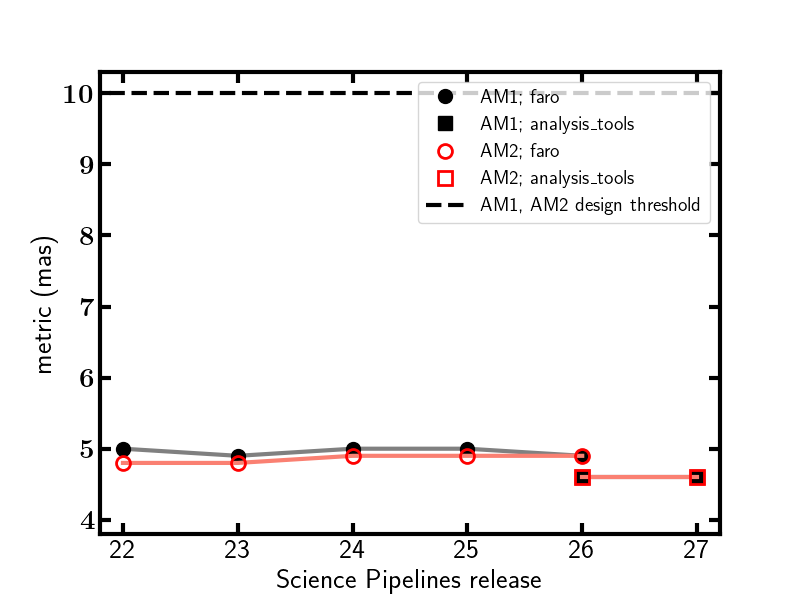
\includegraphics[width=0.475\textwidth, trim=0.0in 0.0in 0.0in 0.0in, clip]{figures/astrom_metrics_v27_with_thresholds.png}
  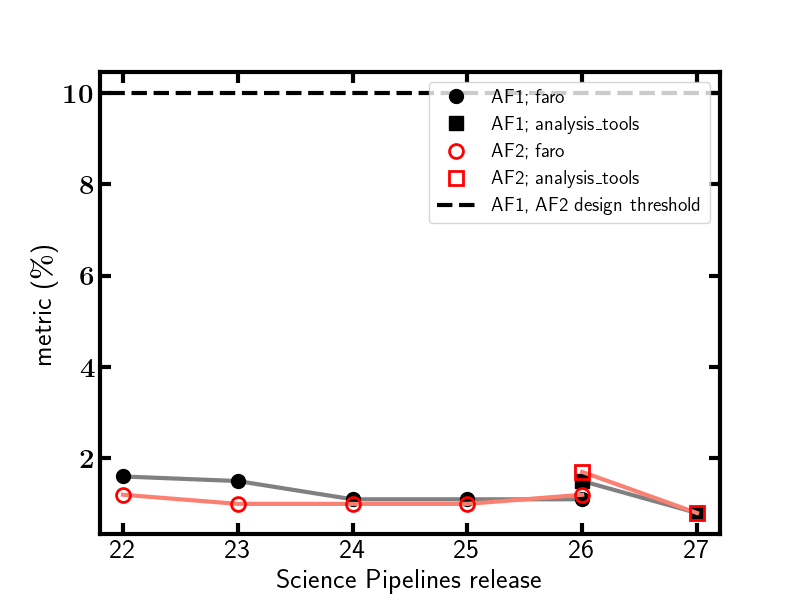
\includegraphics[width=0.475\textwidth, trim=0.0in 0.0in 0.0in 0.0in, clip]{figures/astrom_outlier_metrics_v27_with_thresholds.png}
  \caption{Astrometry metrics measured on $r$-band images compared over the past few major pipelines releases. The figure shows the values of these metrics as measured with \texttt{faro} in versions 22-26 of the LSST Science Pipelines as circles. The measurements from \texttt{analysis\_tools} in versions 26-27 of the Science Pipelines are shown as squares. \textit{Left: } Median astrometric measurement error on 5-arcminute scales (AM1) and 20-arcminute scales (AM2), compared against the SRD requirements (for the ``design'' thresholds; note that the thresholds for AM1 and AM2 are the same, and thus indistinguishable on the figure). \textit{Right: } Fraction of astrometric measurements exceeding the outlier threshold on 5-arcminute (AF1) and 20-arcminute (AF2) scales, compared against the SRD requirements (for the ``design'' thresholds; note that the thresholds for AF1 and AF2 are the same, and thus indistinguishable on the figure). The measured values of the astrometric scatter metrics AM1 and AM2 were virtually unchanged between pipelines version 26 and v27, while the outlier fractions (AF1 and AF2) show some improvement (though this is due to slight algorithmic changes in how they are calculated). }
  \label{fig:astrom_metrics}
\end{figure}

The following metrics are defined following LSR-REQ-0094
\citedsp{LSE-29} and Table 18 of \citeds{LPM-17}. Values in this table represent the mean of the results reported by \texttt{analysis\_tools} for the three tracts in RC2.

Any entries left blank are those for which we do not have data in the given filter for that dataset.

\begin{longtable}[]{@{}llllll@{}}
\toprule
\begin{minipage}[b]{0.12\columnwidth}\raggedright\strut
Metric\strut
\end{minipage} & \begin{minipage}[b]{0.06\columnwidth}\raggedright\strut
Unit\strut
\end{minipage} & \begin{minipage}[b]{0.14\columnwidth}\raggedright\strut
SRD Requirement -- Design\strut
\end{minipage} & \begin{minipage}[b]{0.12\columnwidth}\raggedright\strut
Release 26 Value (RC2)\strut
\end{minipage} & \begin{minipage}[b]{0.12\columnwidth}\raggedright\strut
Release 27 Value (RC2) \strut
\end{minipage} & \begin{minipage}[b]{0.17\columnwidth}\raggedright\strut
Comments\strut
\end{minipage}\tabularnewline
\midrule
\endhead
\begin{minipage}[t]{0.12\columnwidth}\raggedright\strut
AM1: \emph{u}\strut
\end{minipage} & \begin{minipage}[t]{0.06\columnwidth}\raggedright\strut
mas\strut
\end{minipage} & \begin{minipage}[t]{0.14\columnwidth}\raggedright\strut
\(\leq 10\)\strut
\end{minipage} & \begin{minipage}[t]{0.12\columnwidth}\raggedright\strut
---\strut
\end{minipage} & \begin{minipage}[t]{0.12\columnwidth}\raggedright\strut
--- \strut
\end{minipage} & \begin{minipage}[t]{0.17\columnwidth}\raggedright\strut
No data\strut
\end{minipage}\tabularnewline
\begin{minipage}[t]{0.12\columnwidth}\raggedright\strut
AM1: \emph{g}\strut
\end{minipage} & \begin{minipage}[t]{0.06\columnwidth}\raggedright\strut
mas\strut
\end{minipage} & \begin{minipage}[t]{0.14\columnwidth}\raggedright\strut
\(\leq 10\)\strut
\end{minipage} & \begin{minipage}[t]{0.12\columnwidth}\raggedright\strut
5.2\strut
\end{minipage} & \begin{minipage}[t]{0.12\columnwidth}\raggedright\strut
5.2 \strut
\end{minipage} & \begin{minipage}[t]{0.17\columnwidth}\raggedright\strut
\strut
\end{minipage}\tabularnewline
\begin{minipage}[t]{0.12\columnwidth}\raggedright\strut
AM1: \emph{r}\strut
\end{minipage} & \begin{minipage}[t]{0.06\columnwidth}\raggedright\strut
mas\strut
\end{minipage} & \begin{minipage}[t]{0.14\columnwidth}\raggedright\strut
\(\leq 10\)\strut
\end{minipage} & \begin{minipage}[t]{0.12\columnwidth}\raggedright\strut
4.6\strut
\end{minipage} & \begin{minipage}[t]{0.12\columnwidth}\raggedright\strut
4.6\strut
\end{minipage} & \begin{minipage}[t]{0.17\columnwidth}\raggedright\strut
\strut
\end{minipage}\tabularnewline
\begin{minipage}[t]{0.12\columnwidth}\raggedright\strut
AM1: \emph{i}\strut
\end{minipage} & \begin{minipage}[t]{0.06\columnwidth}\raggedright\strut
mas\strut
\end{minipage} & \begin{minipage}[t]{0.14\columnwidth}\raggedright\strut
\(\leq 10\)\strut
\end{minipage} & \begin{minipage}[t]{0.12\columnwidth}\raggedright\strut
4.0\strut
\end{minipage} & \begin{minipage}[t]{0.12\columnwidth}\raggedright\strut
4.1\strut
\end{minipage} & \begin{minipage}[t]{0.17\columnwidth}\raggedright\strut
\strut
\end{minipage}\tabularnewline
\begin{minipage}[t]{0.12\columnwidth}\raggedright\strut
AM1: \emph{z}\strut
\end{minipage} & \begin{minipage}[t]{0.06\columnwidth}\raggedright\strut
mas\strut
\end{minipage} & \begin{minipage}[t]{0.14\columnwidth}\raggedright\strut
\(\leq 10\)\strut
\end{minipage} & \begin{minipage}[t]{0.12\columnwidth}\raggedright\strut
5.2\strut
\end{minipage} & \begin{minipage}[t]{0.12\columnwidth}\raggedright\strut
5.2\strut
\end{minipage} & \begin{minipage}[t]{0.17\columnwidth}\raggedright\strut
\strut
\end{minipage}\tabularnewline
\begin{minipage}[t]{0.12\columnwidth}\raggedright\strut
AM1: \emph{y}\strut
\end{minipage} & \begin{minipage}[t]{0.06\columnwidth}\raggedright\strut
mas\strut
\end{minipage} & \begin{minipage}[t]{0.14\columnwidth}\raggedright\strut
\(\leq 10\)\strut
\end{minipage} & \begin{minipage}[t]{0.12\columnwidth}\raggedright\strut
6.9\strut
\end{minipage} & \begin{minipage}[t]{0.12\columnwidth}\raggedright\strut
6.9\strut
\end{minipage} & \begin{minipage}[t]{0.17\columnwidth}\raggedright\strut
\strut
\end{minipage}\tabularnewline
\begin{minipage}[t]{0.12\columnwidth}\raggedright\strut
AF1: \emph{u}\strut
\end{minipage} & \begin{minipage}[t]{0.06\columnwidth}\raggedright\strut
\%\strut
\end{minipage} & \begin{minipage}[t]{0.14\columnwidth}\raggedright\strut
\(\leq 10\)\strut
\end{minipage} & \begin{minipage}[t]{0.12\columnwidth}\raggedright\strut
---\strut
\end{minipage} & \begin{minipage}[t]{0.12\columnwidth}\raggedright\strut
---\strut
\end{minipage} & \begin{minipage}[t]{0.17\columnwidth}\raggedright\strut
No data\strut
\end{minipage}\tabularnewline
\begin{minipage}[t]{0.12\columnwidth}\raggedright\strut
AF1: \emph{g}\strut
\end{minipage} & \begin{minipage}[t]{0.06\columnwidth}\raggedright\strut
\%\strut
\end{minipage} & \begin{minipage}[t]{0.14\columnwidth}\raggedright\strut
\(\leq 10\)\strut
\end{minipage} & \begin{minipage}[t]{0.12\columnwidth}\raggedright\strut
1.6\strut
\end{minipage} & \begin{minipage}[t]{0.12\columnwidth}\raggedright\strut
0.9\strut
\end{minipage} & \begin{minipage}[t]{0.17\columnwidth}\raggedright\strut
\strut
\end{minipage}\tabularnewline
\begin{minipage}[t]{0.12\columnwidth}\raggedright\strut
AF1: \emph{r}\strut
\end{minipage} & \begin{minipage}[t]{0.06\columnwidth}\raggedright\strut
\%\strut
\end{minipage} & \begin{minipage}[t]{0.14\columnwidth}\raggedright\strut
\(\leq 10\)\strut
\end{minipage} & \begin{minipage}[t]{0.12\columnwidth}\raggedright\strut
1.5\strut
\end{minipage} & \begin{minipage}[t]{0.12\columnwidth}\raggedright\strut
0.8\strut
\end{minipage} & \begin{minipage}[t]{0.17\columnwidth}\raggedright\strut
\strut
\end{minipage}\tabularnewline
\begin{minipage}[t]{0.12\columnwidth}\raggedright\strut
AF1: \emph{i}\strut
\end{minipage} & \begin{minipage}[t]{0.06\columnwidth}\raggedright\strut
\%\strut
\end{minipage} & \begin{minipage}[t]{0.14\columnwidth}\raggedright\strut
\(\leq 10\)\strut
\end{minipage} & \begin{minipage}[t]{0.12\columnwidth}\raggedright\strut
0.9\strut
\end{minipage} & \begin{minipage}[t]{0.12\columnwidth}\raggedright\strut
0.6\strut
\end{minipage} & \begin{minipage}[t]{0.17\columnwidth}\raggedright\strut
\strut
\end{minipage}\tabularnewline
\begin{minipage}[t]{0.12\columnwidth}\raggedright\strut
AF1: \emph{z}\strut
\end{minipage} & \begin{minipage}[t]{0.06\columnwidth}\raggedright\strut
\%\strut
\end{minipage} & \begin{minipage}[t]{0.14\columnwidth}\raggedright\strut
\(\leq 10\)\strut
\end{minipage} & \begin{minipage}[t]{0.12\columnwidth}\raggedright\strut
1.2\strut
\end{minipage} & \begin{minipage}[t]{0.12\columnwidth}\raggedright\strut
0.6\strut
\end{minipage} & \begin{minipage}[t]{0.17\columnwidth}\raggedright\strut
\strut
\end{minipage}\tabularnewline
\begin{minipage}[t]{0.12\columnwidth}\raggedright\strut
AF1: \emph{y}\strut
\end{minipage} & \begin{minipage}[t]{0.06\columnwidth}\raggedright\strut
\%\strut
\end{minipage} & \begin{minipage}[t]{0.14\columnwidth}\raggedright\strut
\(\leq 10\)\strut
\end{minipage} & \begin{minipage}[t]{0.12\columnwidth}\raggedright\strut
3.8\strut
\end{minipage} & \begin{minipage}[t]{0.12\columnwidth}\raggedright\strut
2.9\strut
\end{minipage} & \begin{minipage}[t]{0.17\columnwidth}\raggedright\strut
\strut
\end{minipage}\tabularnewline
\begin{minipage}[t]{0.12\columnwidth}\raggedright\strut
AD1: \emph{u}\strut
\end{minipage} & \begin{minipage}[t]{0.06\columnwidth}\raggedright\strut
mas\strut
\end{minipage} & \begin{minipage}[t]{0.14\columnwidth}\raggedright\strut
\(\leq 20\)\strut
\end{minipage} & \begin{minipage}[t]{0.12\columnwidth}\raggedright\strut
---\strut
\end{minipage} & \begin{minipage}[t]{0.12\columnwidth}\raggedright\strut
---\strut
\end{minipage} & \begin{minipage}[t]{0.17\columnwidth}\raggedright\strut
No data\strut
\end{minipage}\tabularnewline
\begin{minipage}[t]{0.12\columnwidth}\raggedright\strut
AD1: \emph{g}\strut
\end{minipage} & \begin{minipage}[t]{0.06\columnwidth}\raggedright\strut
mas\strut
\end{minipage} & \begin{minipage}[t]{0.14\columnwidth}\raggedright\strut
\(\leq 20\)\strut
\end{minipage} & \begin{minipage}[t]{0.12\columnwidth}\raggedright\strut
10.5\strut
\end{minipage} & \begin{minipage}[t]{0.12\columnwidth}\raggedright\strut
9.7\strut
\end{minipage} & \begin{minipage}[t]{0.17\columnwidth}\raggedright\strut
\strut
\end{minipage}\tabularnewline
\begin{minipage}[t]{0.12\columnwidth}\raggedright\strut
AD1: \emph{r}\strut
\end{minipage} & \begin{minipage}[t]{0.06\columnwidth}\raggedright\strut
mas\strut
\end{minipage} & \begin{minipage}[t]{0.14\columnwidth}\raggedright\strut
\(\leq 20\)\strut
\end{minipage} & \begin{minipage}[t]{0.12\columnwidth}\raggedright\strut
9.7\strut
\end{minipage} & \begin{minipage}[t]{0.12\columnwidth}\raggedright\strut
9.2\strut
\end{minipage} & \begin{minipage}[t]{0.17\columnwidth}\raggedright\strut
\strut
\end{minipage}\tabularnewline
\begin{minipage}[t]{0.12\columnwidth}\raggedright\strut
AD1: \emph{i}\strut
\end{minipage} & \begin{minipage}[t]{0.06\columnwidth}\raggedright\strut
mas\strut
\end{minipage} & \begin{minipage}[t]{0.14\columnwidth}\raggedright\strut
\(\leq 20\)\strut
\end{minipage} & \begin{minipage}[t]{0.12\columnwidth}\raggedright\strut
8.1\strut
\end{minipage} & \begin{minipage}[t]{0.12\columnwidth}\raggedright\strut
7.9\strut
\end{minipage} & \begin{minipage}[t]{0.17\columnwidth}\raggedright\strut
\strut
\end{minipage}\tabularnewline
\begin{minipage}[t]{0.12\columnwidth}\raggedright\strut
AD1: \emph{z}\strut
\end{minipage} & \begin{minipage}[t]{0.06\columnwidth}\raggedright\strut
mas\strut
\end{minipage} & \begin{minipage}[t]{0.14\columnwidth}\raggedright\strut
\(\leq 20\)\strut
\end{minipage} & \begin{minipage}[t]{0.12\columnwidth}\raggedright\strut
10.2\strut
\end{minipage} & \begin{minipage}[t]{0.12\columnwidth}\raggedright\strut
9.7\strut
\end{minipage} & \begin{minipage}[t]{0.17\columnwidth}\raggedright\strut
\strut
\end{minipage}\tabularnewline
\begin{minipage}[t]{0.12\columnwidth}\raggedright\strut
AD1: \emph{y}\strut
\end{minipage} & \begin{minipage}[t]{0.06\columnwidth}\raggedright\strut
mas\strut
\end{minipage} & \begin{minipage}[t]{0.14\columnwidth}\raggedright\strut
\(\leq 20\)\strut
\end{minipage} & \begin{minipage}[t]{0.12\columnwidth}\raggedright\strut
13.3\strut
\end{minipage} & \begin{minipage}[t]{0.12\columnwidth}\raggedright\strut
12.6\strut
\end{minipage} & \begin{minipage}[t]{0.17\columnwidth}\raggedright\strut
\strut
\end{minipage}\tabularnewline
\begin{minipage}[t]{0.12\columnwidth}\raggedright\strut
AM2: \emph{u}\strut
\end{minipage} & \begin{minipage}[t]{0.06\columnwidth}\raggedright\strut
mas\strut
\end{minipage} & \begin{minipage}[t]{0.14\columnwidth}\raggedright\strut
\(\leq 10\)\strut
\end{minipage} & \begin{minipage}[t]{0.12\columnwidth}\raggedright\strut
---\strut
\end{minipage} & \begin{minipage}[t]{0.12\columnwidth}\raggedright\strut
---\strut
\end{minipage} & \begin{minipage}[t]{0.17\columnwidth}\raggedright\strut
No data\strut
\end{minipage}\tabularnewline
\begin{minipage}[t]{0.12\columnwidth}\raggedright\strut
AM2: \emph{g}\strut
\end{minipage} & \begin{minipage}[t]{0.06\columnwidth}\raggedright\strut
mas\strut
\end{minipage} & \begin{minipage}[t]{0.14\columnwidth}\raggedright\strut
\(\leq 10\)\strut
\end{minipage} & \begin{minipage}[t]{0.12\columnwidth}\raggedright\strut
5.3\strut
\end{minipage} & \begin{minipage}[t]{0.12\columnwidth}\raggedright\strut
5.3\strut
\end{minipage} & \begin{minipage}[t]{0.17\columnwidth}\raggedright\strut
\strut
\end{minipage}\tabularnewline
\begin{minipage}[t]{0.12\columnwidth}\raggedright\strut
AM2: \emph{r}\strut
\end{minipage} & \begin{minipage}[t]{0.06\columnwidth}\raggedright\strut
mas\strut
\end{minipage} & \begin{minipage}[t]{0.14\columnwidth}\raggedright\strut
\(\leq 10\)\strut
\end{minipage} & \begin{minipage}[t]{0.12\columnwidth}\raggedright\strut
4.6\strut
\end{minipage} & \begin{minipage}[t]{0.12\columnwidth}\raggedright\strut
4.6\strut
\end{minipage} & \begin{minipage}[t]{0.17\columnwidth}\raggedright\strut
\strut
\end{minipage}\tabularnewline
\begin{minipage}[t]{0.12\columnwidth}\raggedright\strut
AM2: \emph{i}\strut
\end{minipage} & \begin{minipage}[t]{0.06\columnwidth}\raggedright\strut
mas\strut
\end{minipage} & \begin{minipage}[t]{0.14\columnwidth}\raggedright\strut
\(\leq 10\)\strut
\end{minipage} & \begin{minipage}[t]{0.12\columnwidth}\raggedright\strut
4.0\strut
\end{minipage} & \begin{minipage}[t]{0.12\columnwidth}\raggedright\strut
4.0\strut
\end{minipage} & \begin{minipage}[t]{0.17\columnwidth}\raggedright\strut
\strut
\end{minipage}\tabularnewline
\begin{minipage}[t]{0.12\columnwidth}\raggedright\strut
AM2: \emph{z}\strut
\end{minipage} & \begin{minipage}[t]{0.06\columnwidth}\raggedright\strut
mas\strut
\end{minipage} & \begin{minipage}[t]{0.14\columnwidth}\raggedright\strut
\(\leq 10\)\strut
\end{minipage} & \begin{minipage}[t]{0.12\columnwidth}\raggedright\strut
5.2\strut
\end{minipage} & \begin{minipage}[t]{0.12\columnwidth}\raggedright\strut
5.2\strut
\end{minipage} & \begin{minipage}[t]{0.17\columnwidth}\raggedright\strut
\strut
\end{minipage}\tabularnewline
\begin{minipage}[t]{0.12\columnwidth}\raggedright\strut
AM2: \emph{y}\strut
\end{minipage} & \begin{minipage}[t]{0.06\columnwidth}\raggedright\strut
mas\strut
\end{minipage} & \begin{minipage}[t]{0.14\columnwidth}\raggedright\strut
\(\leq 10\)\strut
\end{minipage} & \begin{minipage}[t]{0.12\columnwidth}\raggedright\strut
7.1\strut
\end{minipage} & \begin{minipage}[t]{0.12\columnwidth}\raggedright\strut
7.1\strut
\end{minipage} & \begin{minipage}[t]{0.17\columnwidth}\raggedright\strut
\strut
\end{minipage}\tabularnewline
\begin{minipage}[t]{0.12\columnwidth}\raggedright\strut
AF2: \emph{u}\strut
\end{minipage} & \begin{minipage}[t]{0.06\columnwidth}\raggedright\strut
\%\strut
\end{minipage} & \begin{minipage}[t]{0.14\columnwidth}\raggedright\strut
\(\leq 10\)\strut
\end{minipage} & \begin{minipage}[t]{0.12\columnwidth}\raggedright\strut
---\strut
\end{minipage} & \begin{minipage}[t]{0.12\columnwidth}\raggedright\strut
---\strut
\end{minipage} & \begin{minipage}[t]{0.17\columnwidth}\raggedright\strut
No data\strut
\end{minipage}\tabularnewline
\begin{minipage}[t]{0.12\columnwidth}\raggedright\strut
AF2: \emph{g}\strut
\end{minipage} & \begin{minipage}[t]{0.06\columnwidth}\raggedright\strut
\%\strut
\end{minipage} & \begin{minipage}[t]{0.14\columnwidth}\raggedright\strut
\(\leq 10\)\strut
\end{minipage} & \begin{minipage}[t]{0.12\columnwidth}\raggedright\strut
1.9\strut
\end{minipage} & \begin{minipage}[t]{0.12\columnwidth}\raggedright\strut
0.9\strut
\end{minipage} & \begin{minipage}[t]{0.17\columnwidth}\raggedright\strut
\strut
\end{minipage}\tabularnewline
\begin{minipage}[t]{0.12\columnwidth}\raggedright\strut
AF2: \emph{r}\strut
\end{minipage} & \begin{minipage}[t]{0.06\columnwidth}\raggedright\strut
\%\strut
\end{minipage} & \begin{minipage}[t]{0.14\columnwidth}\raggedright\strut
\(\leq 10\)\strut
\end{minipage} & \begin{minipage}[t]{0.12\columnwidth}\raggedright\strut
1.7\strut
\end{minipage} & \begin{minipage}[t]{0.12\columnwidth}\raggedright\strut
0.8\strut
\end{minipage} & \begin{minipage}[t]{0.17\columnwidth}\raggedright\strut
\strut
\end{minipage}\tabularnewline
\begin{minipage}[t]{0.12\columnwidth}\raggedright\strut
AF2: \emph{i}\strut
\end{minipage} & \begin{minipage}[t]{0.06\columnwidth}\raggedright\strut
\%\strut
\end{minipage} & \begin{minipage}[t]{0.14\columnwidth}\raggedright\strut
\(\leq 10\)\strut
\end{minipage} & \begin{minipage}[t]{0.12\columnwidth}\raggedright\strut
0.9\strut
\end{minipage} & \begin{minipage}[t]{0.12\columnwidth}\raggedright\strut
0.6\strut
\end{minipage} & \begin{minipage}[t]{0.17\columnwidth}\raggedright\strut
\strut
\end{minipage}\tabularnewline
\begin{minipage}[t]{0.12\columnwidth}\raggedright\strut
AF2: \emph{z}\strut
\end{minipage} & \begin{minipage}[t]{0.06\columnwidth}\raggedright\strut
\%\strut
\end{minipage} & \begin{minipage}[t]{0.14\columnwidth}\raggedright\strut
\(\leq 10\)\strut
\end{minipage} & \begin{minipage}[t]{0.12\columnwidth}\raggedright\strut
1.3\strut
\end{minipage} & \begin{minipage}[t]{0.12\columnwidth}\raggedright\strut
0.7\strut
\end{minipage} & \begin{minipage}[t]{0.17\columnwidth}\raggedright\strut
\strut
\end{minipage}\tabularnewline
\begin{minipage}[t]{0.12\columnwidth}\raggedright\strut
AF2: \emph{y}\strut
\end{minipage} & \begin{minipage}[t]{0.06\columnwidth}\raggedright\strut
\%\strut
\end{minipage} & \begin{minipage}[t]{0.14\columnwidth}\raggedright\strut
\(\leq 10\)\strut
\end{minipage} & \begin{minipage}[t]{0.12\columnwidth}\raggedright\strut
4.3\strut
\end{minipage} & \begin{minipage}[t]{0.12\columnwidth}\raggedright\strut
3.3\strut
\end{minipage} & \begin{minipage}[t]{0.17\columnwidth}\raggedright\strut
\strut
\end{minipage}\tabularnewline
\begin{minipage}[t]{0.12\columnwidth}\raggedright\strut
AD2: \emph{u}\strut
\end{minipage} & \begin{minipage}[t]{0.06\columnwidth}\raggedright\strut
mas\strut
\end{minipage} & \begin{minipage}[t]{0.14\columnwidth}\raggedright\strut
\(\leq 20\)\strut
\end{minipage} & \begin{minipage}[t]{0.12\columnwidth}\raggedright\strut
---\strut
\end{minipage} & \begin{minipage}[t]{0.12\columnwidth}\raggedright\strut
---\strut
\end{minipage} & \begin{minipage}[t]{0.17\columnwidth}\raggedright\strut
No data\strut
\end{minipage}\tabularnewline
\begin{minipage}[t]{0.12\columnwidth}\raggedright\strut
AD2: \emph{g}\strut
\end{minipage} & \begin{minipage}[t]{0.06\columnwidth}\raggedright\strut
mas\strut
\end{minipage} & \begin{minipage}[t]{0.14\columnwidth}\raggedright\strut
\(\leq 20\)\strut
\end{minipage} & \begin{minipage}[t]{0.12\columnwidth}\raggedright\strut
10.9\strut
\end{minipage} & \begin{minipage}[t]{0.12\columnwidth}\raggedright\strut
10.0\strut
\end{minipage} & \begin{minipage}[t]{0.17\columnwidth}\raggedright\strut
\strut
\end{minipage}\tabularnewline
\begin{minipage}[t]{0.12\columnwidth}\raggedright\strut
AD2: \emph{r}\strut
\end{minipage} & \begin{minipage}[t]{0.06\columnwidth}\raggedright\strut
mas\strut
\end{minipage} & \begin{minipage}[t]{0.14\columnwidth}\raggedright\strut
\(\leq 20\)\strut
\end{minipage} & \begin{minipage}[t]{0.12\columnwidth}\raggedright\strut
10.0\strut
\end{minipage} & \begin{minipage}[t]{0.12\columnwidth}\raggedright\strut
9.3\strut
\end{minipage} & \begin{minipage}[t]{0.17\columnwidth}\raggedright\strut
\strut
\end{minipage}\tabularnewline
\begin{minipage}[t]{0.12\columnwidth}\raggedright\strut
AD2: \emph{i}\strut
\end{minipage} & \begin{minipage}[t]{0.06\columnwidth}\raggedright\strut
mas\strut
\end{minipage} & \begin{minipage}[t]{0.14\columnwidth}\raggedright\strut
\(\leq 20\)\strut
\end{minipage} & \begin{minipage}[t]{0.12\columnwidth}\raggedright\strut
8.1\strut
\end{minipage} & \begin{minipage}[t]{0.12\columnwidth}\raggedright\strut
7.9\strut
\end{minipage} & \begin{minipage}[t]{0.17\columnwidth}\raggedright\strut
\strut
\end{minipage}\tabularnewline
\begin{minipage}[t]{0.12\columnwidth}\raggedright\strut
AD2: \emph{z}\strut
\end{minipage} & \begin{minipage}[t]{0.06\columnwidth}\raggedright\strut
mas\strut
\end{minipage} & \begin{minipage}[t]{0.14\columnwidth}\raggedright\strut
\(\leq 20\)\strut
\end{minipage} & \begin{minipage}[t]{0.12\columnwidth}\raggedright\strut
10.5\strut
\end{minipage} & \begin{minipage}[t]{0.12\columnwidth}\raggedright\strut
9.9\strut
\end{minipage} & \begin{minipage}[t]{0.17\columnwidth}\raggedright\strut
\strut
\end{minipage}\tabularnewline
\begin{minipage}[t]{0.12\columnwidth}\raggedright\strut
AD2: \emph{y}\strut
\end{minipage} & \begin{minipage}[t]{0.06\columnwidth}\raggedright\strut
mas\strut
\end{minipage} & \begin{minipage}[t]{0.14\columnwidth}\raggedright\strut
\(\leq 20\)\strut
\end{minipage} & \begin{minipage}[t]{0.12\columnwidth}\raggedright\strut
13.7\strut
\end{minipage} & \begin{minipage}[t]{0.12\columnwidth}\raggedright\strut
12.9\strut
\end{minipage} & \begin{minipage}[t]{0.17\columnwidth}\raggedright\strut
\strut
\end{minipage}\tabularnewline
%\begin{minipage}[t]{0.12\columnwidth}\raggedright\strut
%AB1: \emph{u}\strut
%\end{minipage} & \begin{minipage}[t]{0.06\columnwidth}\raggedright\strut
%mas\strut
%\end{minipage} & \begin{minipage}[t]{0.14\columnwidth}\raggedright\strut
%\(\leq 10\)\strut
%\end{minipage} & \begin{minipage}[t]{0.12\columnwidth}\raggedright\strut
%---\strut
%\end{minipage} & \begin{minipage}[t]{0.12\columnwidth}\raggedright\strut
%---\strut
%\end{minipage} & \begin{minipage}[t]{0.17\columnwidth}\raggedright\strut
%No data\strut
%\end{minipage}\tabularnewline
%\begin{minipage}[t]{0.12\columnwidth}\raggedright\strut
%AB1: \emph{g}\strut
%\end{minipage} & \begin{minipage}[t]{0.06\columnwidth}\raggedright\strut
%mas\strut
%\end{minipage} & \begin{minipage}[t]{0.14\columnwidth}\raggedright\strut
%\(\leq 10\)\strut
%\end{minipage} & \begin{minipage}[t]{0.12\columnwidth}\raggedright\strut
%4.9\strut
%\end{minipage} & \begin{minipage}[t]{0.12\columnwidth}\raggedright\strut
%5.1\strut
%\end{minipage} & \begin{minipage}[t]{0.17\columnwidth}\raggedright\strut
%\strut
%\end{minipage}\tabularnewline
%\begin{minipage}[t]{0.12\columnwidth}\raggedright\strut
%AB1: \emph{r}\strut
%\end{minipage} & \begin{minipage}[t]{0.06\columnwidth}\raggedright\strut
%mas\strut
%\end{minipage} & \begin{minipage}[t]{0.14\columnwidth}\raggedright\strut
%\(\leq 10\)\strut
%\end{minipage} & \begin{minipage}[t]{0.12\columnwidth}\raggedright\strut
%4.7\strut
%\end{minipage} & \begin{minipage}[t]{0.12\columnwidth}\raggedright\strut
%4.8\strut
%\end{minipage} & \begin{minipage}[t]{0.17\columnwidth}\raggedright\strut
%\strut
%\end{minipage}\tabularnewline
%\begin{minipage}[t]{0.12\columnwidth}\raggedright\strut
%AB1: \emph{i}\strut
%\end{minipage} & \begin{minipage}[t]{0.06\columnwidth}\raggedright\strut
%mas\strut
%\end{minipage} & \begin{minipage}[t]{0.14\columnwidth}\raggedright\strut
%\(\leq 10\)\strut
%\end{minipage} & \begin{minipage}[t]{0.12\columnwidth}\raggedright\strut
%5.7\strut
%\end{minipage} & \begin{minipage}[t]{0.12\columnwidth}\raggedright\strut
%6.0\strut
%\end{minipage} & \begin{minipage}[t]{0.17\columnwidth}\raggedright\strut
%\strut
%\end{minipage}\tabularnewline
%\begin{minipage}[t]{0.12\columnwidth}\raggedright\strut
%AB1: \emph{z}\strut
%\end{minipage} & \begin{minipage}[t]{0.06\columnwidth}\raggedright\strut
%mas\strut
%\end{minipage} & \begin{minipage}[t]{0.14\columnwidth}\raggedright\strut
%\(\leq 10\)\strut
%\end{minipage} & \begin{minipage}[t]{0.12\columnwidth}\raggedright\strut
%4.9\strut
%\end{minipage} & \begin{minipage}[t]{0.12\columnwidth}\raggedright\strut
%4.8\strut
%\end{minipage} & \begin{minipage}[t]{0.17\columnwidth}\raggedright\strut
%\strut
%\end{minipage}\tabularnewline
%\begin{minipage}[t]{0.12\columnwidth}\raggedright\strut
%AB1: \emph{y}\strut
%\end{minipage} & \begin{minipage}[t]{0.06\columnwidth}\raggedright\strut
%mas\strut
%\end{minipage} & \begin{minipage}[t]{0.14\columnwidth}\raggedright\strut
%\(\leq 10\)\strut
%\end{minipage} & \begin{minipage}[t]{0.12\columnwidth}\raggedright\strut
%7.0\strut
%\end{minipage} & \begin{minipage}[t]{0.12\columnwidth}\raggedright\strut
%7.2\strut
%\end{minipage} & \begin{minipage}[t]{0.17\columnwidth}\raggedright\strut
%\strut
%\end{minipage}\tabularnewline
\bottomrule
\end{longtable}

\section{Ellipticity Correlations}\label{ellipticity-correlations}

\begin{figure}[!t]
  \centering
  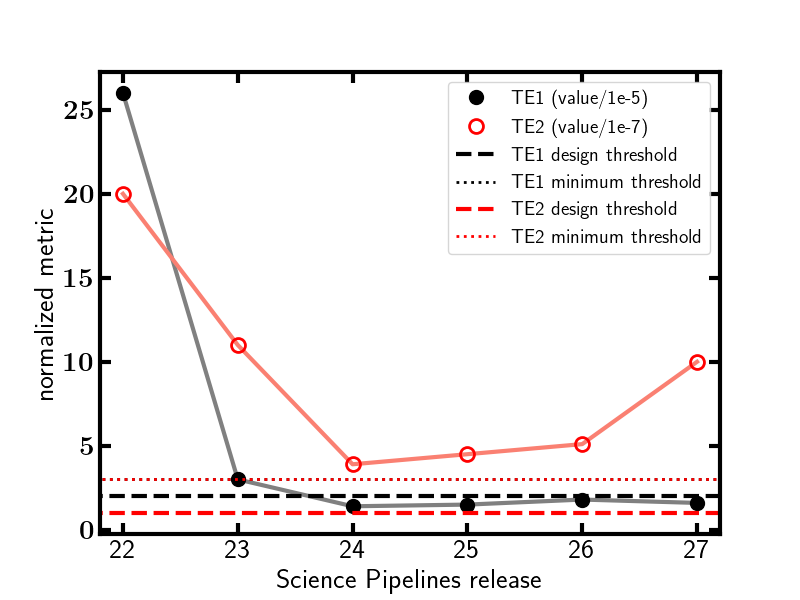
\includegraphics[width=0.6\textwidth, trim=0.0in 0.0in 0.0in 0.0in, clip]{figures/ellip_metrics_v27_with_thresholds.png}
  \caption{Median ellipticity residual correlations at 1-arcminute (TE1; normalized by a factor of $1\times10^{-5}$) and 5-arcminute (TE2; normalized by $1\times10^{-7}$) scales, as measured on $r$-band images, compared over the past few major pipelines releases. Measurements are compared against the SRD requirements (for both the ``design'' and ``minimum'' thresholds; note that the normalized minimum thresholds for TE1 and TE2 are the same, and thus indistinguishable on the figure). TE1 shows a slight improvement between v26 and v27, whereas TE2 increased significantly. At present, we don't believe TE1 and TE2 are adequately capturing changes to our PSFs, so we are actively working on a revised definition of those metrics to be implemented in `analysis\_tools`. As mentioned in the text, we made changes to the PSF modeling input star selection criteria that likely contributed to changes in TE1 and TE2. We are looking into these, but we suspect the metric definitions are noisy and the significance of the regression is unclear.}
  \label{fig:ellip_metrics}
\end{figure}

The following metrics are defined following LSR-REQ-0097
\citedsp{LSE-29} and Table 27 of \citeds{LPM-17}. Values in this table represent the mean of the results reported by \texttt{faro} for the three tracts in RC2.

Any entries left blank are those for which we do not have data in the given filter for that dataset.

\begin{longtable}[]{@{}llllll@{}}
\toprule
\begin{minipage}[b]{0.12\columnwidth}\raggedright\strut
Metric\strut
\end{minipage} & \begin{minipage}[b]{0.06\columnwidth}\raggedright\strut
Unit\strut
\end{minipage} & \begin{minipage}[b]{0.14\columnwidth}\raggedright\strut
SRD Requirement -- Design\strut
\end{minipage} & \begin{minipage}[b]{0.12\columnwidth}\raggedright\strut
Release 26 Value (RC2) \strut
\end{minipage} & \begin{minipage}[b]{0.12\columnwidth}\raggedright\strut
Release 27 Value (RC2) \strut
\end{minipage} & \begin{minipage}[b]{0.17\columnwidth}\raggedright\strut
Comments\strut
\end{minipage}\tabularnewline
\midrule
\endhead
\begin{minipage}[t]{0.12\columnwidth}\raggedright\strut
TE1: \emph{u}\strut
\end{minipage} & \begin{minipage}[t]{0.06\columnwidth}\raggedright\strut
---\strut
\end{minipage} & \begin{minipage}[t]{0.14\columnwidth}\raggedright\strut
\(\leq 2\times10^{-5}\)\strut
\end{minipage} & \begin{minipage}[t]{0.12\columnwidth}\raggedright\strut
---\strut
\end{minipage} & \begin{minipage}[t]{0.12\columnwidth}\raggedright\strut
--- \strut
\end{minipage} & \begin{minipage}[t]{0.17\columnwidth}\raggedright\strut
No data\strut
\end{minipage}\tabularnewline
\begin{minipage}[t]{0.12\columnwidth}\raggedright\strut
TE1: \emph{g}\strut
\end{minipage} & \begin{minipage}[t]{0.06\columnwidth}\raggedright\strut
---\strut
\end{minipage} & \begin{minipage}[t]{0.14\columnwidth}\raggedright\strut
\(\leq 2\times10^{-5}\)\strut
\end{minipage} & \begin{minipage}[t]{0.12\columnwidth}\raggedright\strut
\(1.8\times10^{-5}\) \strut
\end{minipage} & \begin{minipage}[t]{0.12\columnwidth}\raggedright\strut
\(1.6\times10^{-5}\) \strut
\end{minipage} & \begin{minipage}[t]{0.17\columnwidth}\raggedright\strut
\strut
\end{minipage}\tabularnewline
\begin{minipage}[t]{0.12\columnwidth}\raggedright\strut
TE1: \emph{r}\strut
\end{minipage} & \begin{minipage}[t]{0.06\columnwidth}\raggedright\strut
---\strut
\end{minipage} & \begin{minipage}[t]{0.14\columnwidth}\raggedright\strut
\(\leq 2\times10^{-5}\)\strut
\end{minipage} & \begin{minipage}[t]{0.12\columnwidth}\raggedright\strut
\(1.8\times10^{-5}\)\strut
\end{minipage} & \begin{minipage}[t]{0.12\columnwidth}\raggedright\strut
\(1.6\times10^{-5}\)\strut
\end{minipage} & \begin{minipage}[t]{0.17\columnwidth}\raggedright\strut
\strut
\end{minipage}\tabularnewline
\begin{minipage}[t]{0.12\columnwidth}\raggedright\strut
TE1: \emph{i}\strut
\end{minipage} & \begin{minipage}[t]{0.06\columnwidth}\raggedright\strut
---\strut
\end{minipage} & \begin{minipage}[t]{0.14\columnwidth}\raggedright\strut
\(\leq 2\times10^{-5}\)\strut
\end{minipage} & \begin{minipage}[t]{0.12\columnwidth}\raggedright\strut
\(1.3\times10^{-5}\)\strut
\end{minipage} & \begin{minipage}[t]{0.12\columnwidth}\raggedright\strut
\(2.1\times10^{-5}\)\strut
\end{minipage} & \begin{minipage}[t]{0.17\columnwidth}\raggedright\strut
\strut
\end{minipage}\tabularnewline
\begin{minipage}[t]{0.12\columnwidth}\raggedright\strut
TE1: \emph{z}\strut
\end{minipage} & \begin{minipage}[t]{0.06\columnwidth}\raggedright\strut
---\strut
\end{minipage} & \begin{minipage}[t]{0.14\columnwidth}\raggedright\strut
\(\leq 2\times10^{-5}\)\strut
\end{minipage} & \begin{minipage}[t]{0.12\columnwidth}\raggedright\strut
\(1.1\times10^{-5}\) \strut
\end{minipage} & \begin{minipage}[t]{0.12\columnwidth}\raggedright\strut
\(1.3\times10^{-5}\)\strut
\end{minipage} & \begin{minipage}[t]{0.17\columnwidth}\raggedright\strut
\strut
\end{minipage}\tabularnewline
\begin{minipage}[t]{0.12\columnwidth}\raggedright\strut
TE1: \emph{y}\strut
\end{minipage} & \begin{minipage}[t]{0.06\columnwidth}\raggedright\strut
---\strut
\end{minipage} & \begin{minipage}[t]{0.14\columnwidth}\raggedright\strut
\(\leq 2\times10^{-5}\)\strut
\end{minipage} & \begin{minipage}[t]{0.12\columnwidth}\raggedright\strut
\(2.5\times10^{-5}\)\strut
\end{minipage} & \begin{minipage}[t]{0.12\columnwidth}\raggedright\strut
\(6.4\times10^{-5}\)\strut
\end{minipage} & \begin{minipage}[t]{0.17\columnwidth}\raggedright\strut
\strut
\end{minipage}\tabularnewline
\begin{minipage}[t]{0.12\columnwidth}\raggedright\strut
TE2: \emph{u}\strut
\end{minipage} & \begin{minipage}[t]{0.06\columnwidth}\raggedright\strut
---\strut
\end{minipage} & \begin{minipage}[t]{0.14\columnwidth}\raggedright\strut
\(\leq 1\times10^{-7}\)\strut
\end{minipage} & \begin{minipage}[t]{0.12\columnwidth}\raggedright\strut
---\strut
\end{minipage} & \begin{minipage}[t]{0.12\columnwidth}\raggedright\strut
---\strut
\end{minipage} & \begin{minipage}[t]{0.17\columnwidth}\raggedright\strut
No data\strut
\end{minipage}\tabularnewline
\begin{minipage}[t]{0.12\columnwidth}\raggedright\strut
TE2: \emph{g}\strut
\end{minipage} & \begin{minipage}[t]{0.06\columnwidth}\raggedright\strut
---\strut
\end{minipage} & \begin{minipage}[t]{0.14\columnwidth}\raggedright\strut
\(\leq 1\times10^{-7}\)\strut
\end{minipage} & \begin{minipage}[t]{0.12\columnwidth}\raggedright\strut
\(6.4\times10^{-7}\)\strut
\end{minipage} & \begin{minipage}[t]{0.12\columnwidth}\raggedright\strut
\(7.0\times10^{-7}\)\strut
\end{minipage} & \begin{minipage}[t]{0.17\columnwidth}\raggedright\strut
\strut
\end{minipage}\tabularnewline
\begin{minipage}[t]{0.12\columnwidth}\raggedright\strut
TE2: \emph{r}\strut
\end{minipage} & \begin{minipage}[t]{0.06\columnwidth}\raggedright\strut
---\strut
\end{minipage} & \begin{minipage}[t]{0.14\columnwidth}\raggedright\strut
\(\leq 1\times10^{-7}\)\strut
\end{minipage} & \begin{minipage}[t]{0.12\columnwidth}\raggedright\strut
\(5.1\times10^{-7}\)\strut
\end{minipage} & \begin{minipage}[t]{0.12\columnwidth}\raggedright\strut
\(1.0\times10^{-6}\)\strut
\end{minipage} & \begin{minipage}[t]{0.17\columnwidth}\raggedright\strut
\strut
\end{minipage}\tabularnewline
\begin{minipage}[t]{0.12\columnwidth}\raggedright\strut
TE2: \emph{i}\strut
\end{minipage} & \begin{minipage}[t]{0.06\columnwidth}\raggedright\strut
---\strut
\end{minipage} & \begin{minipage}[t]{0.14\columnwidth}\raggedright\strut
\(\leq 1\times10^{-7}\)\strut
\end{minipage} & \begin{minipage}[t]{0.12\columnwidth}\raggedright\strut
\(4.7\times10^{-7}\)\strut
\end{minipage} & \begin{minipage}[t]{0.12\columnwidth}\raggedright\strut
\(6.7\times10^{-7}\)\strut
\end{minipage} & \begin{minipage}[t]{0.17\columnwidth}\raggedright\strut
\strut
\end{minipage}\tabularnewline
\begin{minipage}[t]{0.12\columnwidth}\raggedright\strut
TE2: \emph{z}\strut
\end{minipage} & \begin{minipage}[t]{0.06\columnwidth}\raggedright\strut
---\strut
\end{minipage} & \begin{minipage}[t]{0.14\columnwidth}\raggedright\strut
\(\leq 1\times10^{-7}\)\strut
\end{minipage} & \begin{minipage}[t]{0.12\columnwidth}\raggedright\strut
\(3.2\times10^{-7}\)\strut
\end{minipage} & \begin{minipage}[t]{0.12\columnwidth}\raggedright\strut
\(6.1\times10^{-7}\)\strut
\end{minipage} & \begin{minipage}[t]{0.17\columnwidth}\raggedright\strut
\strut
\end{minipage}\tabularnewline
\begin{minipage}[t]{0.12\columnwidth}\raggedright\strut
TE2: \emph{y}\strut
\end{minipage} & \begin{minipage}[t]{0.06\columnwidth}\raggedright\strut
---\strut
\end{minipage} & \begin{minipage}[t]{0.14\columnwidth}\raggedright\strut
\(\leq 1\times10^{-7}\)\strut
\end{minipage} & \begin{minipage}[t]{0.12\columnwidth}\raggedright\strut
\(8.8\times10^{-7}\)\strut
\end{minipage} & \begin{minipage}[t]{0.12\columnwidth}\raggedright\strut
\(1.1\times10^{-6}\)\strut
\end{minipage} & \begin{minipage}[t]{0.17\columnwidth}\raggedright\strut
\strut
\end{minipage}\tabularnewline
\bottomrule
\end{longtable}

\section{Computational Performance}\label{computational-performance}

Computational performance metrics were not measured for this release.

\appendix

% Include all the relevant bib files.
% https://lsst-texmf.lsst.io/lsstdoc.html#bibliographies
\section{References} \label{sec:bib}
\renewcommand{\refname}{} % Suppress default Bibliography section
\bibliography{local,lsst,lsst-dm,refs_ads,refs,books}

% Make sure lsst-texmf/bin/generateAcronyms.py is in your path
\section{Acronyms} \label{sec:acronyms}
\addtocounter{table}{-1}
\begin{longtable}{p{0.145\textwidth}p{0.8\textwidth}}\hline
\textbf{Acronym} & \textbf{Description}  \\\hline

CCD & Charge-Coupled Device \\\hline
DM & Data Management \\\hline
DMSR & DM System Requirements; LSE-61 \\\hline
DMTN & DM Technical Note \\\hline
DMTR & DM Test Report \\\hline
DRP & Data Release Production \\\hline
FAQ & Frequently Asked Question \\\hline
HSC & Hyper Suprime-Cam \\\hline
HSC-SSP & HSC Subaru Strategic Program \\\hline
KPM & Key Performance Metric \\\hline
LPM & LSST Project Management (Document Handle) \\\hline
LSE & LSST Systems Engineering (Document Handle) \\\hline
LSR & LSST System Requirements; LSE-29 \\\hline
LSST & Legacy Survey of Space and Time (formerly Large Synoptic Survey Telescope) \\\hline
PSF & Point Spread Function \\\hline
Pan-STARRS & Panoramic Survey Telescope and Rapid Response System \\\hline
SRD & LSST Science Requirements; LPM-17 \\\hline
\end{longtable}

% If you want glossary uncomment below and comment out the two lines above.
% \printglossaries

\end{document}
